% ============================================================
%  Relatório Técnico – Aprendizagem de Máquina Clássica
%  QSAR Biodegradation – UNEB
% ============================================================
\documentclass[12pt, a4paper]{article}

% --- Codificação e língua ---
\usepackage[brazil]{babel}

% --- Fontes e tipografia ---
\usepackage{fontspec}
\usepackage{microtype}

% --- Layout ---
\usepackage[top=2.5cm, bottom=2.5cm, left=3cm, right=2.5cm]{geometry}
\usepackage{setspace}
\onehalfspacing

% --- Figuras e tabelas ---
\usepackage{graphicx}
\usepackage{float}
\usepackage{booktabs}
\usepackage{longtable}
\usepackage{tabularx}
\usepackage{multirow}
\usepackage{caption}
\captionsetup{font=small, labelfont=bf}
\graphicspath{{../figs/}}

% --- Cores e links ---
\usepackage[dvipsnames]{xcolor}
\usepackage[hidelinks]{hyperref}

% --- Cabeçalho e rodapé ---
\usepackage{fancyhdr}
\pagestyle{fancy}
\fancyhf{}
\rhead{\small QSAR Biodegradation}
\lhead{\small Aprendizagem de Máquina Clássica}
\rfoot{\small Página \thepage}
\renewcommand{\headrulewidth}{0.4pt}

% --- Código inline ---
\usepackage{listings}
\lstset{basicstyle=\ttfamily\small, backgroundcolor=\color{gray!10},
        frame=single, breaklines=true}

% --- Referências ---
\usepackage[round]{natbib}

% ============================================================
\begin{document}

% ── Capa ────────────────────────────────────────────────────
\begin{titlepage}
  \centering
  \vspace*{1.5cm}
  {\large \textbf{UNIVERSIDADE DO ESTADO DA BAHIA}\\[0.3cm]}
  {\normalsize Departamento de Ciências Exatas e da Terra\\[2cm]}

  {\Large \textbf{Aprendizagem de Máquina Clássica}\\[0.5cm]}
  {\large Trabalho Prático 2\\[2cm]}

  {\LARGE \textbf{Predição de Biodegradabilidade Molecular\\
  com Técnicas de Aprendizado de Máquina Clássica}\\[0.5cm]}
  {\large Dataset: QSAR Biodegradation\\[3cm]}

  \begin{flushleft}
    \textbf{Alunos:}\\[0.3cm]
    Caio Seixas de Melo\\
    Gabriel Cerqueira Santos Rodrigues\\
    Luiz Vinícius Pereira de Oliveira Souza\\
    Luiza de Sá Florentino Limoeiro\\[2cm]
  \end{flushleft}

  \vfill
  {\normalsize Salvador, \the\year}
\end{titlepage}

% ── Sumário ─────────────────────────────────────────────────
\tableofcontents
\newpage

% ============================================================
\section{Apresentação do Dataset}
% ============================================================

O dataset de biodegradação QSAR foi construído pelo Grupo de Pesquisa em
Quimiometria e QSAR de Milão \citep{mansouri2013}. O conjunto de dados contém
valores para 41 atributos (descritores moleculares) utilizados para classificar
substâncias químicas em duas classes: \textit{prontamente biodegradável} (RB) e
\textit{não prontamente biodegradável} (NRB). Após remoção de duplicatas e
registros com valores ausentes, o dataset final conta com \textbf{1.052 amostras
válidas}.

Em relação à distribuição das classes, o dataset apresenta desbalanceamento
moderado: 699 amostras pertencem à classe NRB (66,4\%) e 353 amostras à classe
RB (33,6\%), conforme ilustrado na Figura~\ref{fig:classes}. Essa proporção
aproximada de 2:1 é relevante para as decisões de pré-processamento,
especialmente a escolha do SMOTE para balanceamento durante o treinamento.

\begin{figure}[H]
  \centering
  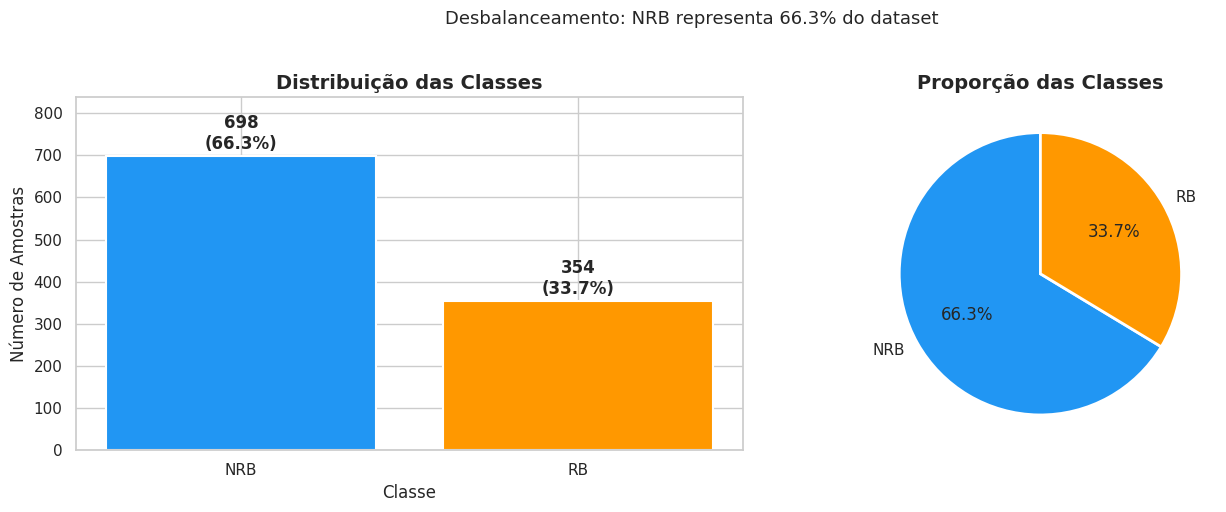
\includegraphics[width=0.92\textwidth]{fig_01_distribuicao_classes}
  \caption{Distribuição das classes RB e NRB no dataset QSAR Biodegradation.}
  \label{fig:classes}
\end{figure}

Os 41 descritores moleculares cobrem propriedades topológicas, eletrônicas e
estruturais das moléculas, conforme listado na Tabela~\ref{tab:descritores}.

\begin{longtable}{clp{9cm}}
\caption{Descritores moleculares do dataset QSAR Biodegradation.}
\label{tab:descritores} \\
\toprule
\textbf{\#} & \textbf{Nome} & \textbf{Descrição} \\
\midrule
\endfirsthead
\multicolumn{3}{c}{\small\textit{Tabela~\ref{tab:descritores} -- continuação}} \\
\toprule
\textbf{\#} & \textbf{Nome} & \textbf{Descrição} \\
\midrule
\endhead
\midrule
\multicolumn{3}{r}{\small\textit{continua na próxima página}} \\
\endfoot
\bottomrule
\endlastfoot
1  & SpMax\_L      & Autovalor principal da matriz de Laplace \\
2  & J\_Dz(e)      & Índice tipo Balaban (matriz de Barysz / eletronegatividade) \\
3  & nHM           & Número de átomos pesados \\
4  & F01[N-N]      & Frequência de N-N na distância topológica 1 \\
5  & F04[C-N]      & Frequência de C-N na distância topológica 4 \\
6  & NssssC        & Número de átomos do tipo ssssC \\
7  & nCb-          & Número de C(sp2) substituídos no benzeno \\
8  & C\%           & Percentagem de átomos de C \\
9  & nCp           & Número de C(sp3) primários terminais \\
10 & nO            & Número de átomos de oxigênio \\
11 & F03[C-N]      & Frequência de C-N na distância topológica 3 \\
12 & SdssC         & Soma dos estados E de dssC \\
13 & HyWi\_B(m)   & Índice hiper-Wiener (logarítmico) da matriz de Burden (massa) \\
14 & LOC           & Índice cêntrico de Lopping \\
15 & SM6\_L        & Momento espectral de ordem 6 da matriz de Laplace \\
16 & F03[C-O]      & Frequência de C-O na distância topológica 3 \\
17 & Me            & Eletronegatividade média de Sanderson (escalonada) \\
18 & Mi            & Primeiro potencial de ionização médio (escalonado) \\
19 & nN-N          & Número de N hidrazinas \\
20 & nArNO2        & Número de grupos nitro aromáticos \\
21 & nCRX3         & Número de CRX3 \\
22 & SpPosA\_B(p)  & Soma espectral positiva normalizada (Burden / polarizabilidade) \\
23 & nCIR          & Número de circuitos \\
24 & B01[C-Br]     & Presença/ausência de C-Br na distância topológica 1 \\
25 & B03[C-Cl]     & Presença/ausência de C-Cl na distância topológica 3 \\
26 & N-073         & Ar2NH / Ar3N / Ar2N-Al / R..N..R \\
27 & SpMax\_A      & Autovalor principal da matriz de adjacência (Lovasz-Pelikan) \\
28 & Psi\_i\_1d    & Índice de pseudoconectividade do estado intrínseco (tipo 1d) \\
29 & B04[C-Br]     & Presença/ausência de C-Br na distância topológica 4 \\
30 & SdO           & Soma dos estados E de dO \\
31 & TI2\_L        & Segundo índice de Mohar da matriz de Laplace \\
32 & nCrt          & Número de C(sp3) terciários do anel \\
33 & C-026         & R-{}-CX-{}-R \\
34 & F02[C-N]      & Frequência de C-N na distância topológica 2 \\
35 & nHDon         & Número de doadores de ligações de hidrogênio (N e O) \\
36 & SpMax\_B(m)   & Autovalor principal da matriz de Burden (massa) \\
37 & Psi\_i\_A     & Índice de pseudoconectividade do estado intrínseco (média S) \\
38 & nN            & Número de átomos de nitrogênio \\
39 & SM6\_B(m)     & Momento espectral de ordem 6 da matriz de Burden (massa) \\
40 & nArCOOR       & Número de ésteres aromáticos \\
41 & nX            & Número de átomos de halogênio \\
42 & Classe experimental & prontamente biodegradável (RB) e não prontamente biodegradável (NRB) \\
\bottomrule
\end{longtable}

% ============================================================
\section{Análise e Preparação dos Dados}
% ============================================================

O pré-processamento seguiu uma sequência rígida para evitar vazamento de
informações: (1) EDA sobre o dataset completo; (2) divisão treino/teste;
(3) seleção de features; (4) remoção de outliers; (5) normalização Z-Score;
(6) balanceamento SMOTE por fold. Cada etapa é descrita a seguir.

\subsection{Análise Exploratória dos Dados (EDA)}

Antes de qualquer transformação, foi conduzida uma Análise Exploratória dos
Dados (EDA) sobre o conjunto original completo. A distribuição das 12 features
de maior variância por classe é apresentada na Figura~\ref{fig:features_var}, e
o mapa de correlação das 20 features de maior variância na
Figura~\ref{fig:corr_var}.

\begin{figure}[H]
  \centering
  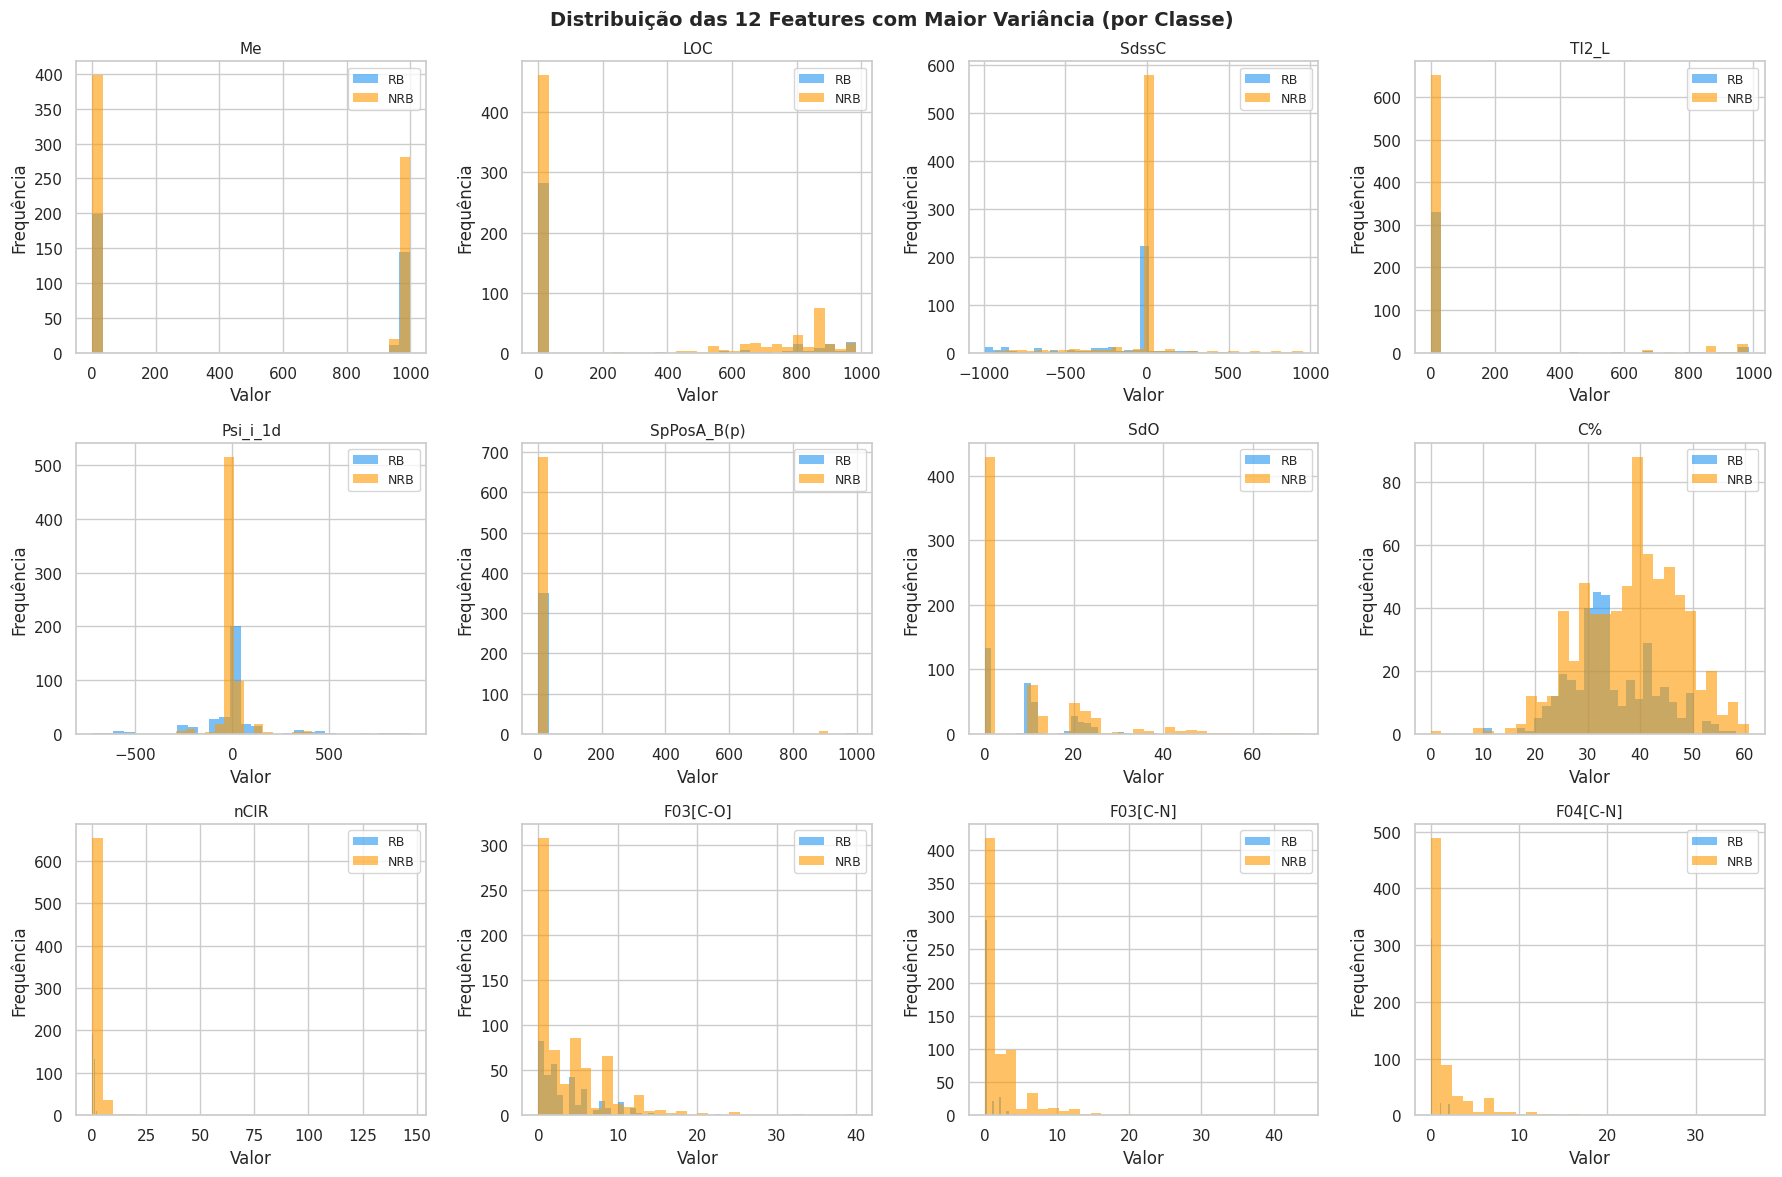
\includegraphics[width=\textwidth]{fig_02_distribuicao_features}
  \caption{Distribuição das 12 features com maior variância, separadas por classe.}
  \label{fig:features_var}
\end{figure}

\begin{figure}[H]
  \centering
  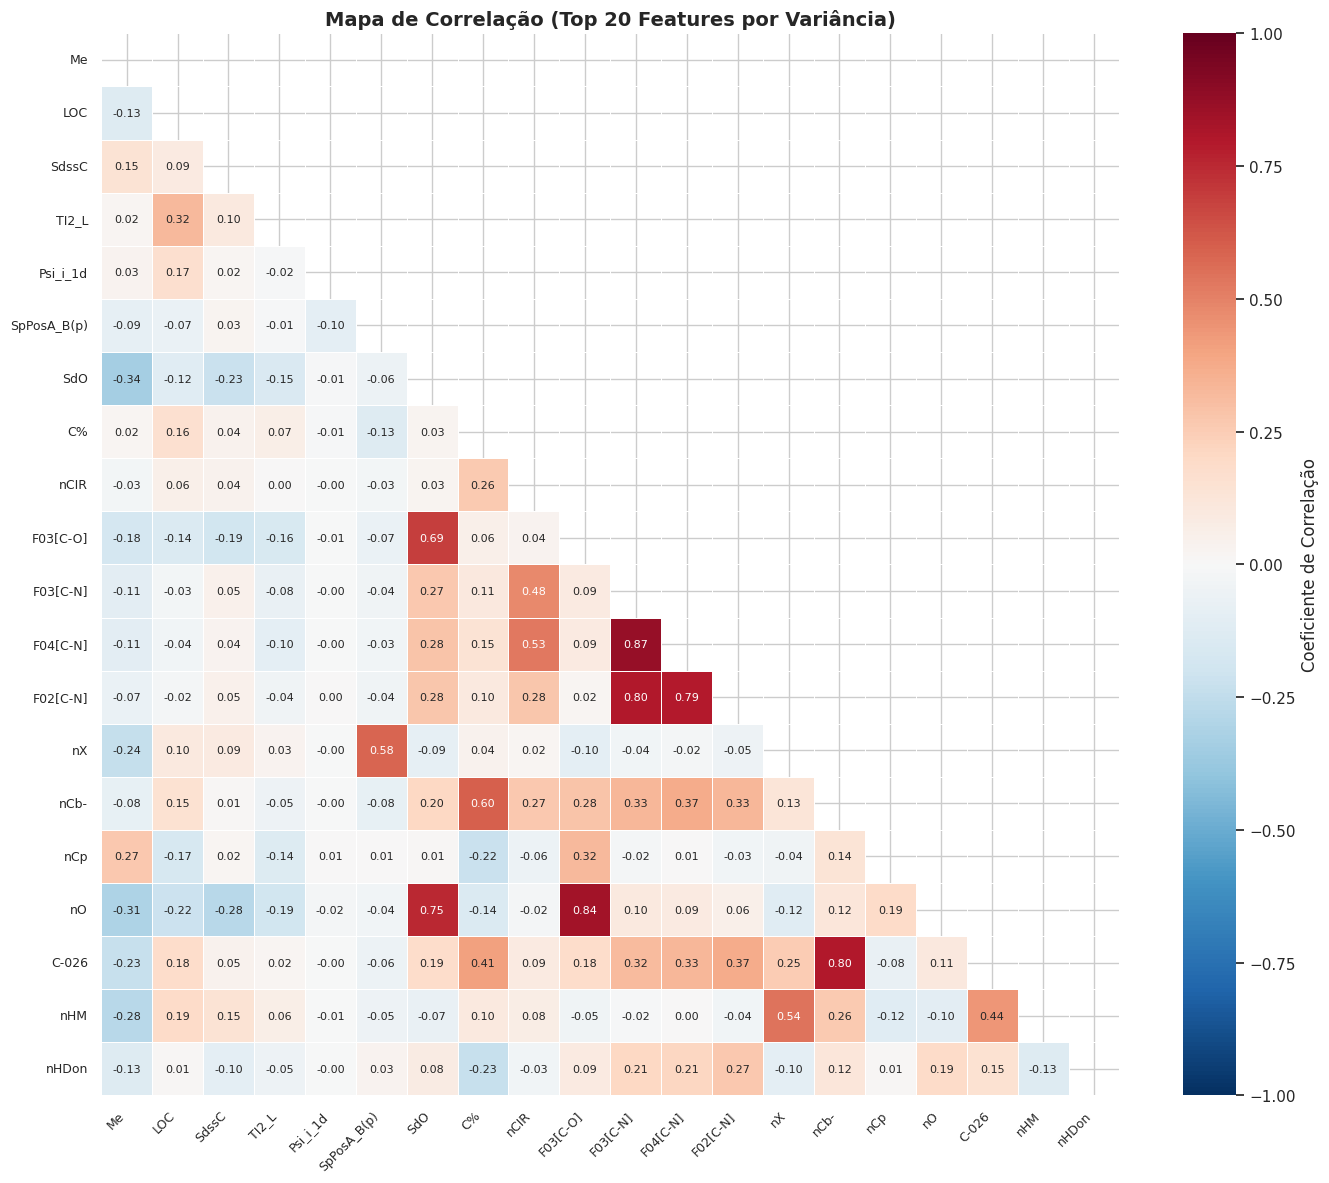
\includegraphics[width=0.92\textwidth]{fig_03_correlacao_variancia}
  \caption{EDA --- Mapa de correlação das 20 features com \textbf{maior variância} (conjunto completo, antes da seleção de features).}
  \label{fig:corr_var}
\end{figure}

A EDA confirmou ausência de valores nulos ou duplicatas e identificou pares de
features altamente correlacionados entre as variáveis de maior variância, como
F03[C-N] $\times$ F04[C-N] com $r = 0{,}87$ e F03[C-O] $\times$ nO com
$r = 0{,}84$. Importante notar que este mapa cobre as features de maior variância,
não necessariamente as mais discriminativas --- a análise do conjunto efetivamente
selecionado para os modelos é apresentada na Seção~\ref{sec:features}.

\subsection{Limpeza e Codificação}

O dataset foi carregado e passou por limpeza: remoção de registros duplicados e
de amostras com valores faltantes. A verificação confirmou ausência de nulos,
tornando desnecessária qualquer imputação. A variável alvo
(\textit{experimental class}) foi convertida para valores numéricos via
\textit{Label Encoding} (NRB = 0, RB = 1).

\subsection{Divisão Treino/Teste}

Os dados foram divididos em treinamento (80\%) e teste (20\%) de forma
estratificada, preservando a proporção original das classes em ambos os
subconjuntos. O conjunto de teste foi completamente isolado desde esse momento,
sem participar de nenhuma etapa subsequente de transformação ou ajuste.

\subsection{Seleção de Features}
\label{sec:features}

Foi treinado um modelo \textit{Random Forest} com \texttt{class\_weight=
"balanced"} exclusivamente sobre os dados de treinamento para identificar os 20
atributos mais relevantes. A importância calculada pelo modelo é apresentada na
Figura~\ref{fig:importancia_rf}. A redução de 41 para 20 features elimina
atributos pouco informativos, reduz o custo computacional e melhora a
generalização dos modelos.

\begin{figure}[H]
  \centering
  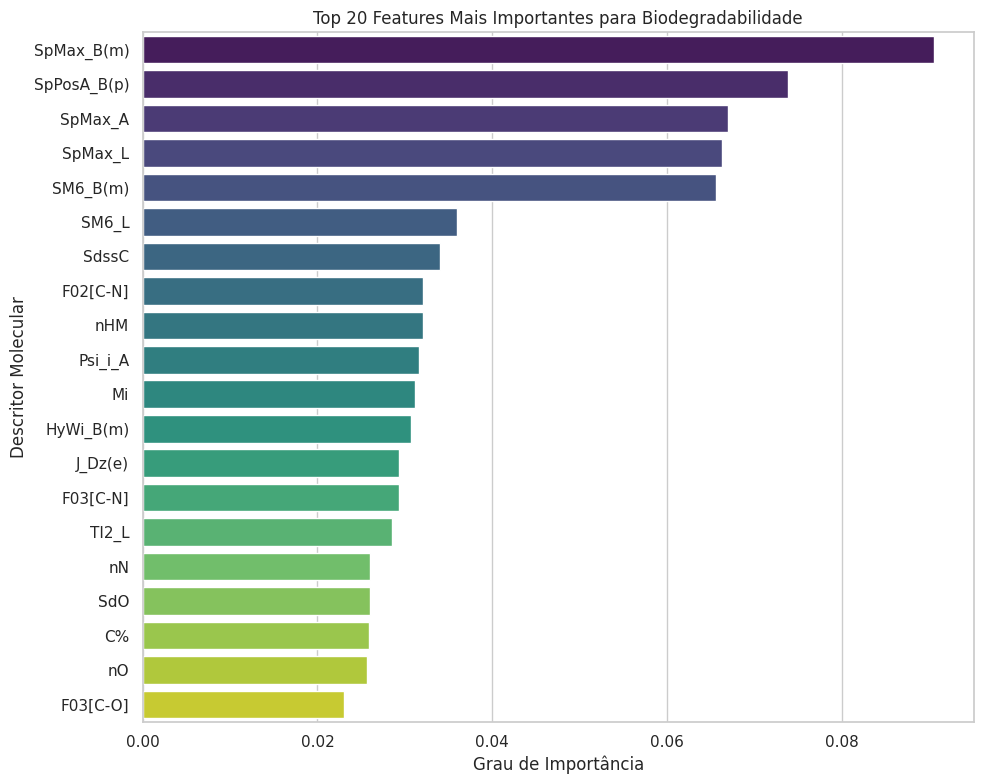
\includegraphics[width=0.82\textwidth]{fig_04_importancia_rf}
  \caption{Top 20 features por importância no \textit{Random Forest}.}
  \label{fig:importancia_rf}
\end{figure}

O mapa de correlação das features efetivamente selecionadas
(Figura~\ref{fig:corr_rf}) revelou alta colinearidade na família de índices
espectrais SpMax/SM6: as features SpMax\_B(m), SpMax\_L, SpMax\_A, SM6\_B(m) e
SM6\_L apresentam correlações superiores a $r = 0{,}91$ entre si. Vale notar
que o conjunto de features selecionado por importância RF e o conjunto de maior
variância se sobrepõem em apenas 50\%, evidenciando que variância e relevância
preditiva são conceitos distintos.

\begin{figure}[H]
  \centering
  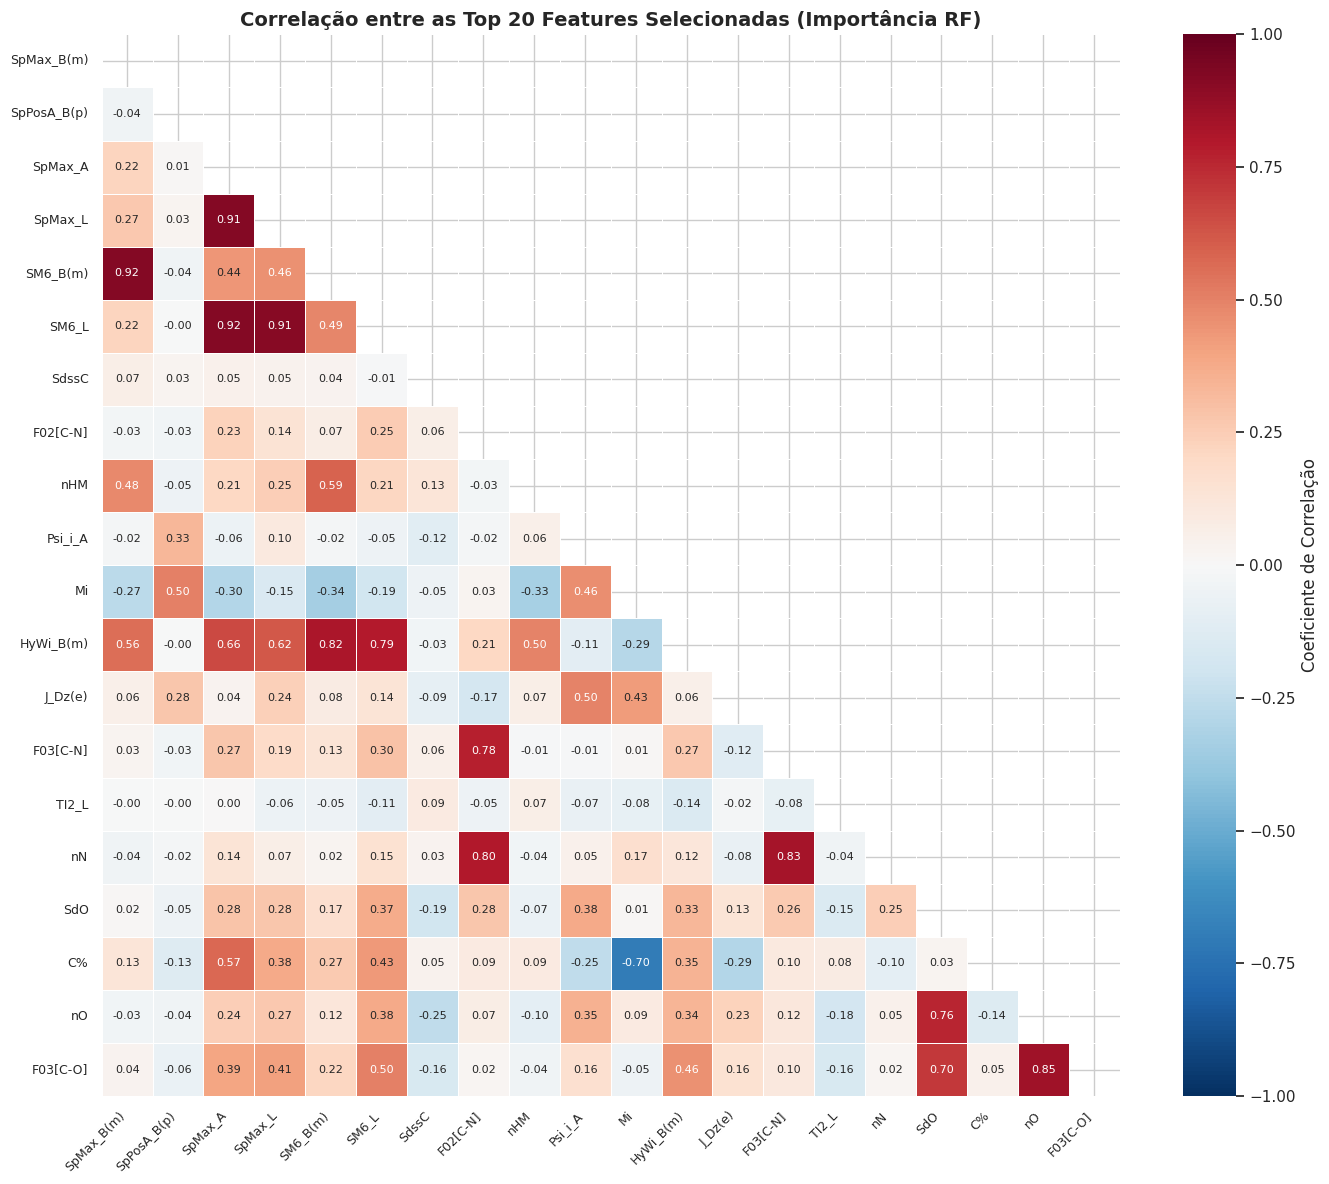
\includegraphics[width=0.92\textwidth]{fig_05_correlacao_rf}
  \caption{Mapa de correlação entre as 20 features \textbf{selecionadas por importância RF} (conjunto de treino, após seleção). Note que este conjunto difere em 50\% das features de maior variância.}
  \label{fig:corr_rf}
\end{figure}

\subsection{Remoção de Outliers}

O algoritmo \textit{Isolation Forest} foi aplicado com parâmetro de contaminação
de 5\% exclusivamente sobre o conjunto de treinamento, removendo 42 amostras
anômalas ($\approx 5\%$) e reduzindo o treino de 841 para 799 amostras. O
conjunto de teste foi preservado integralmente.

\subsection{Normalização}

Os dados foram normalizados pelo método Z-Score (\texttt{StandardScaler}):
média e desvio padrão calculados exclusivamente sobre o treino limpo, aplicados
passivamente ao teste. A normalização é crítica para o KNN (distâncias) e para
a MLP (gradientes).

\subsection{Balanceamento (SMOTE)}

O \textit{SMOTE} foi integrado a um pipeline do \texttt{imbalanced-learn} e
aplicado dinamicamente em cada dobra do 5-Fold Cross Validation, garantindo que
amostras sintéticas nunca contaminem o fold de validação durante a busca de
hiperparâmetros.

% ============================================================
\section{Definição do Protocolo Experimental}
% ============================================================

Os dados foram divididos estratificadamente em 80\% para treinamento e 20\% para
teste. O conjunto de teste foi isolado desde o início e utilizado exclusivamente
na avaliação final.

A validação dos hiperparâmetros foi conduzida via \textbf{5-Fold Cross
Validation} dentro do conjunto de treinamento. Em cada dobra, o pipeline
executou automaticamente: (1) aplicação do SMOTE apenas nos dados de treino da
dobra e (2) treinamento do classificador com a configuração avaliada. Essa
estratégia elimina o risco de vazamento entre treino e validação, pois as
amostras sintéticas são geradas com dados exclusivos de cada iteração.

A busca de hiperparâmetros foi realizada por \textit{Grid Search} exaustivo.
O critério de seleção foi o \textbf{F1-Score Macro} médio das cinco dobras,
escolhido por penalizar igualmente erros em ambas as classes
independentemente do desbalanceamento.

Após identificar os melhores hiperparâmetros, o modelo otimizado foi treinado
sobre todo o conjunto de treinamento e avaliado no conjunto de teste. Por nunca
ter participado de nenhuma etapa de ajuste, os resultados no teste representam
uma estimativa confiável da capacidade de generalização.

% ============================================================
\section{Modelagem Supervisionada}
% ============================================================

Foram utilizados três algoritmos com características distintas de aprendizado,
permitindo comparações entre abordagens baseadas em regras, proximidade e
aprendizado não linear.

\subsection{Árvore de Decisão}

A Árvore de Decisão foi escolhida por sua interpretabilidade e capacidade de
capturar relações não lineares por meio de divisões hierárquicas dos dados.
Os hiperparâmetros otimizados foram: \texttt{criterion} (Gini ou Entropia),
\texttt{max\_depth}, \texttt{min\_samples\_split}, \texttt{min\_samples\_leaf}
e \texttt{class\_weight}.

\subsection{K-Nearest Neighbors}

O KNN classifica amostras com base na classe majoritária entre os $k$ vizinhos
mais próximos no espaço de features. Foram otimizados: \texttt{n\_neighbors},
\texttt{weights} (uniforme ou ponderado por distância) e \texttt{metric}
(Euclidiana ou Manhattan).

\subsection{Rede Neural Artificial (MLP)}

O MLP foi escolhido por sua capacidade de modelar relações altamente não
lineares. Os hiperparâmetros otimizados foram: \texttt{hidden\_layer\_sizes}
(arquiteturas com 1 e 2 camadas ocultas), \texttt{activation} (ReLU, tanh,
logistic), \texttt{alpha} (regularização L2) e \texttt{learning\_rate\_init}.

\subsection{Hiperparâmetros Selecionados}

Após o GridSearchCV com 5-Fold CV, os melhores hiperparâmetros encontrados
foram:

\begin{table}[H]
\centering
\caption{Melhores hiperparâmetros selecionados por GridSearchCV.}
\label{tab:hiperparametros}
\small
\begin{tabularx}{\textwidth}{lX}
\toprule
\textbf{Modelo} & \textbf{Hiperparâmetros} \\
\midrule
Árvore de Decisão &
  \texttt{criterion=entropy, max\_depth=15,}\\
  & \texttt{min\_samples\_leaf=1, min\_samples\_split=10} \\
\addlinespace
KNN &
  \texttt{metric=euclidean, n\_neighbors=5, weights=distance} \\
\addlinespace
MLP &
  \texttt{activation=relu, hidden\_layer\_sizes=(50,),}\\
  & \texttt{alpha=0.1, learning\_rate\_init=0.001} \\
\bottomrule
\end{tabularx}
\end{table}

Destaca-se que a MLP selecionada é deliberadamente simples e regularizada
(\texttt{alpha=0,1}): o 5-Fold CV identificou sobreajuste nas arquiteturas
maiores testadas. O KNN com $k=5$ e distância Euclidiana reflete a estrutura
local dos dados após normalização Z-Score.

% ============================================================
\section{Modelagem Não Supervisionada}
% ============================================================

\subsection{Preparação dos Dados para o K-Means}

Para a trilha não supervisionada foi preparado um dataset exclusivo, partindo
das 20 features selecionadas pelo Random Forest no conjunto de treinamento
(80\%). O Isolation Forest (contaminação = 5\%) foi aplicado de forma
independente, resultando em 799 amostras limpas. Uma normalização Z-Score
própria foi ajustada sobre esse subconjunto. Todo o processo ocorreu sem acesso
aos rótulos, preservando o caráter não supervisionado.

\subsection{Escolha do Número de Clusters}

Para determinar $k$, foram utilizados dois critérios em conjunto com $k$
variando de 2 a 10 (Figura~\ref{fig:cotovelo}).

\begin{figure}[H]
  \centering
  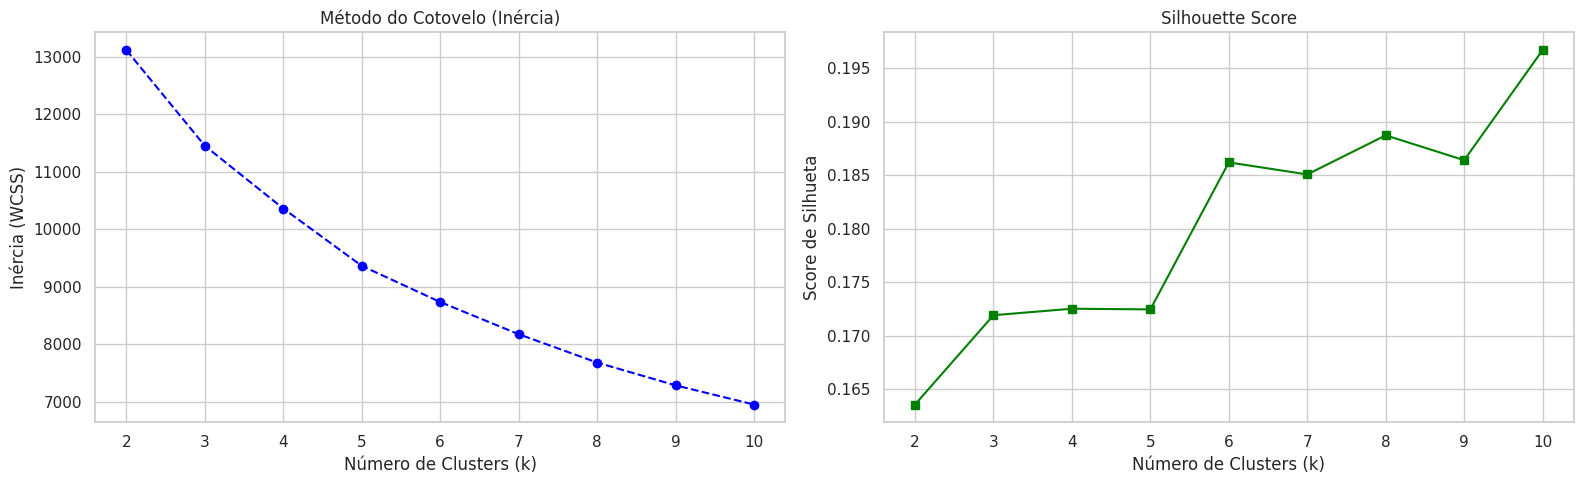
\includegraphics[width=\textwidth]{fig_09_cotovelo_silhouette}
  \caption{Método do Cotovelo (inércia) e Silhouette Score para $k = 2$ a $10$.}
  \label{fig:cotovelo}
\end{figure}

\textbf{Método do Cotovelo:} a curva de inércia decresce suavemente de $k=2$
a $k=10$, sem cotovelo nítido. As maiores quedas ocorrem nas transições
$k=2 \to 3$ e $k=3 \to 4$.

\textbf{Silhouette Score:} os valores são baixos em toda a faixa
(máximo $\approx 0{,}172$ em $k=5$), refletindo sobreposição natural entre
as classes moleculares. Nenhum $k$ domina claramente os demais.

\textbf{Decisão:} adotou-se $\mathbf{k=2}$ como escolha principal por três
razões: (i) o problema é originalmente binário (RB vs.\ NRB), e testar se o
K-Means recupera essa estrutura sem supervisão é a pergunta central da análise;
(ii) $k=2$ corresponde à maior redução de inércia; (iii) os silhouette scores
são próximos ao longo de toda a faixa, sem dominante claro. Como análise
complementar, executou-se também $k=5$ (melhor silhouette local).

\subsection{Resultados do K-Means}

\begin{table}[H]
\centering
\caption{Métricas do K-Means para $k=2$ (principal) e $k=5$ (complementar).}
\label{tab:kmeans}
\begin{tabular}{lcc}
\toprule
$k$ & Inércia & Silhouette \\
\midrule
2 (principal)    & 13.114,2 & 0,1635 \\
5 (complementar) &  9.363,5 & 0,1724 \\
\bottomrule
\end{tabular}
\end{table}

Para $k=2$, a tabela de contingência entre clusters e classes reais revelou:

\begin{table}[H]
\centering
\caption{Tabela de contingência: clusters K-Means ($k=2$) vs.\ classes reais.}
\label{tab:contingencia}
\begin{tabular}{lcc}
\toprule
               & \textbf{Cluster 0} & \textbf{Cluster 1} \\
\midrule
NRB            & 169                & 354                \\
RB             & 193                &  83                \\
\addlinespace
Classe majoritária & RB (53,3\%)   & NRB (81,0\%)       \\
\bottomrule
\end{tabular}
\end{table}

O Cluster 1 concentrou 81,0\% das amostras NRB, indicando que moléculas não
biodegradáveis compartilham padrões moleculares distintivos detectáveis sem
supervisão. A visualização PCA dos clusters é apresentada na
Figura~\ref{fig:pca}, e a análise dos centroides nas
Figuras~\ref{fig:centroides_heat} e \ref{fig:centroides_diff}.

\begin{figure}[H]
  \centering
  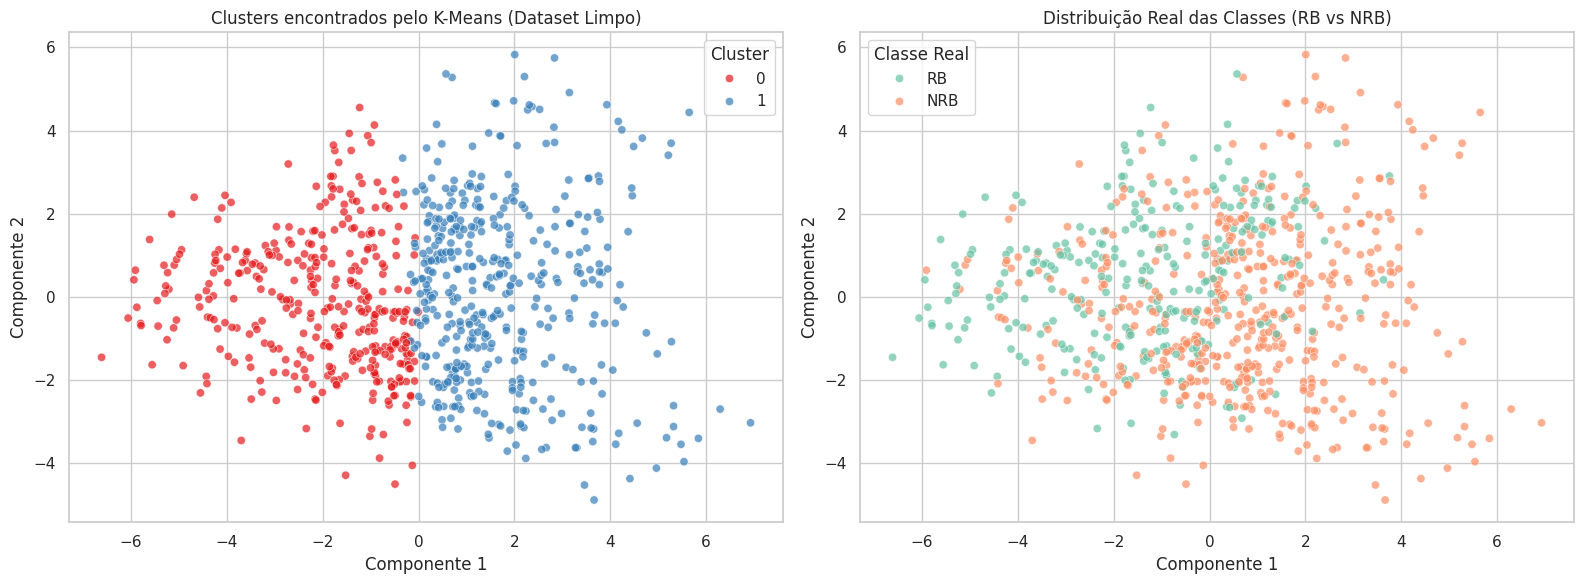
\includegraphics[width=\textwidth]{fig_10_pca_clusters}
  \caption{Projeção PCA 2D dos clusters K-Means (esq.) e classes reais (dir.).}
  \label{fig:pca}
\end{figure}

\begin{figure}[H]
  \centering
  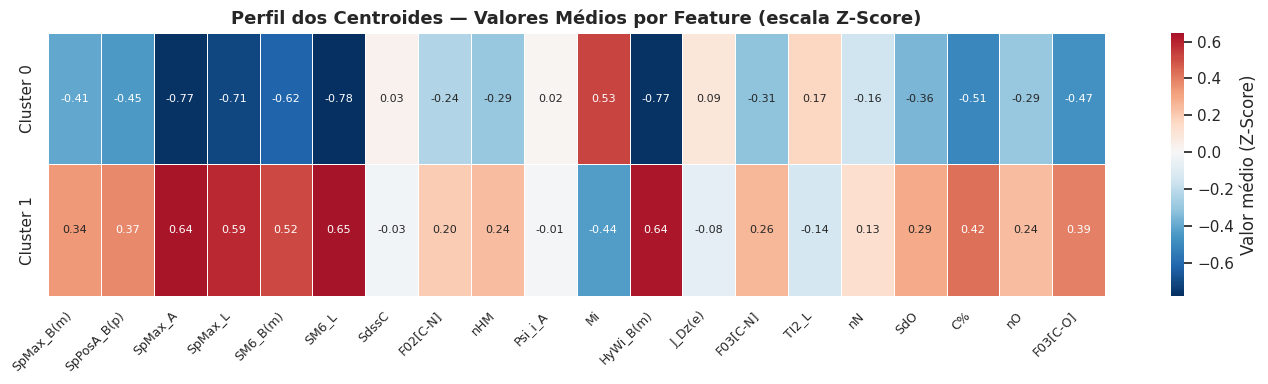
\includegraphics[width=\textwidth]{fig_11_centroides_heatmap}
  \caption{Perfil dos centroides dos clusters em escala Z-Score.}
  \label{fig:centroides_heat}
\end{figure}

\begin{figure}[H]
  \centering
  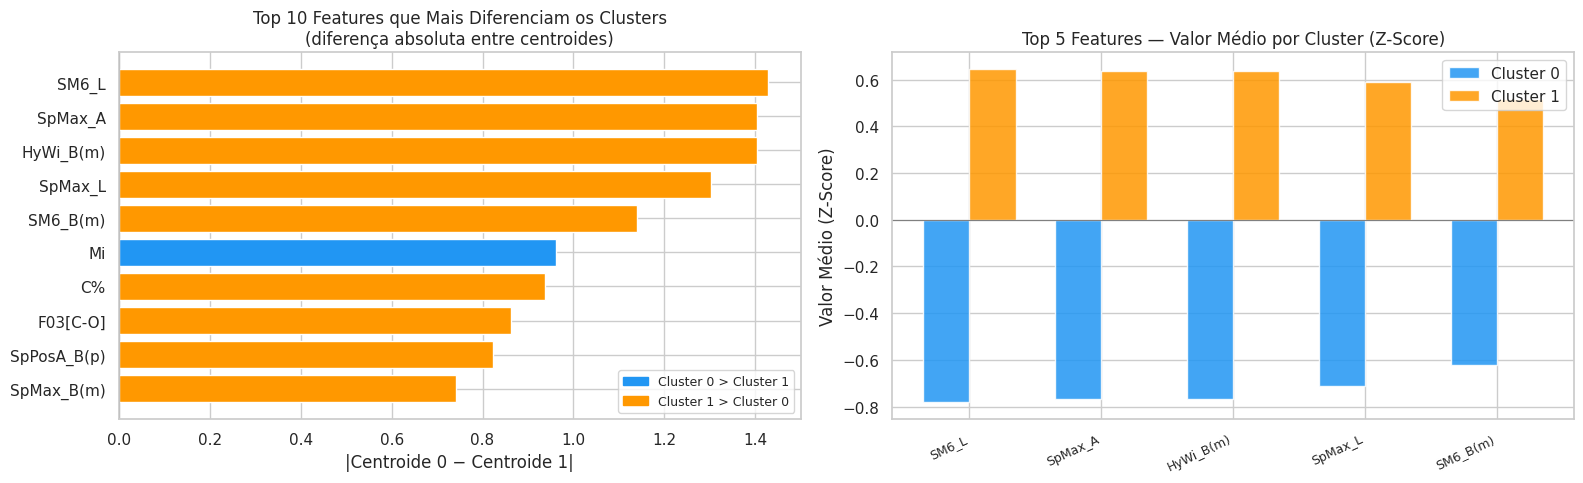
\includegraphics[width=\textwidth]{fig_12_centroides_diff}
  \caption{Features que mais diferenciam os clusters (diferença absoluta entre centroides).}
  \label{fig:centroides_diff}
\end{figure}

% ============================================================
\section{Resultados}
% ============================================================

\subsection{Modelos Supervisionados}

Os modelos foram avaliados sobre o conjunto de teste (211 amostras: 140 NRB
e 71 RB). A Tabela~\ref{tab:resultados} consolida as métricas obtidas.

\begin{table}[H]
\centering
\caption{Comparativo dos modelos supervisionados no conjunto de teste.}
\label{tab:resultados}
\begin{tabular}{lcccccc}
\toprule
\textbf{Modelo} & \textbf{Acurácia} & \textbf{F1-Macro} & \textbf{F1-NRB} & \textbf{F1-RB} & \textbf{Recall-M.} & \textbf{AUC-ROC} \\
\midrule
Árvore de Decisão & 80,6\% & 0,782 & 0,854 & 0,709 & 0,781 & 0,801 \\
KNN               & 83,0\% & 0,820 & 0,862 & 0,778 & 0,844 & 0,907 \\
MLP               & \textbf{85,3\%} & \textbf{0,838} & \textbf{0,889} & \textbf{0,789} & 0,844 & 0,901 \\
\bottomrule
\end{tabular}
\end{table}

As matrizes de confusão individuais são apresentadas na
Figura~\ref{fig:confusion_matrices}, as curvas ROC na
Figura~\ref{fig:roc} e o gráfico radar comparativo na
Figura~\ref{fig:radar}.

\begin{figure}[H]
  \centering
  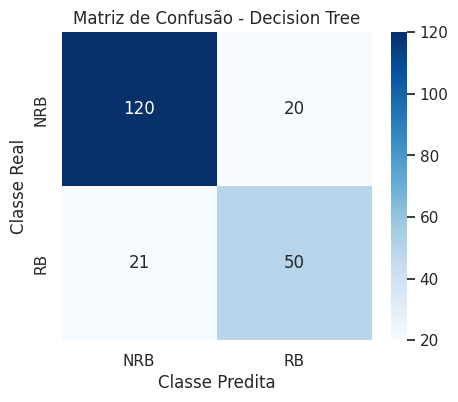
\includegraphics[width=0.32\textwidth]{fig_06_cm_dt}
  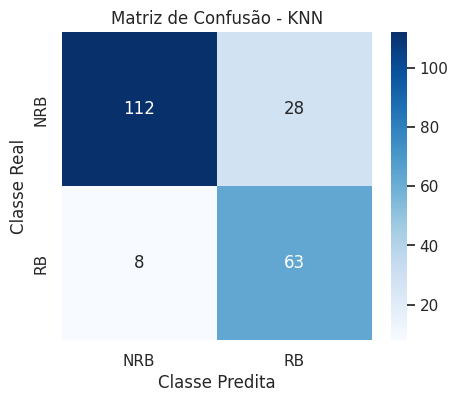
\includegraphics[width=0.32\textwidth]{fig_07_cm_knn}
  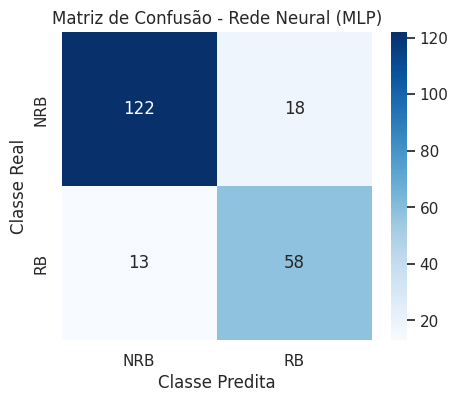
\includegraphics[width=0.32\textwidth]{fig_08_cm_mlp}
  \caption{Matrizes de confusão: Árvore de Decisão (esq.), KNN (centro) e MLP (dir.).}
  \label{fig:confusion_matrices}
\end{figure}

\begin{figure}[H]
  \centering
  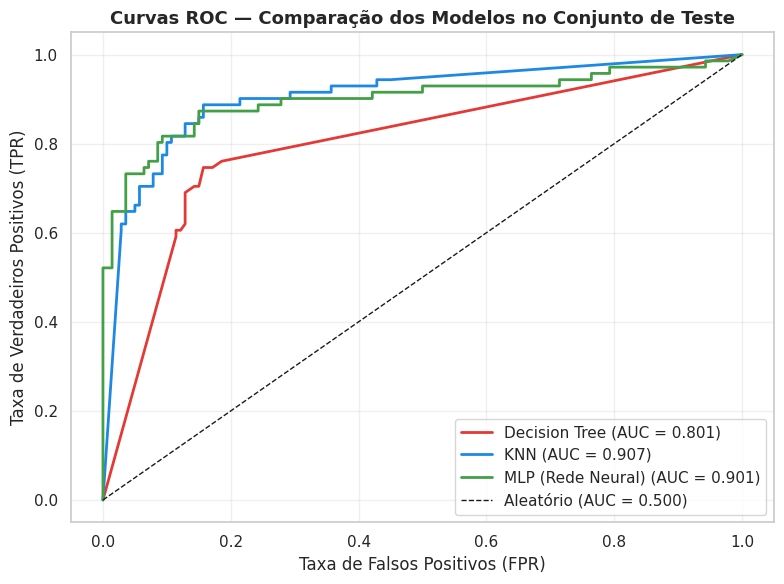
\includegraphics[width=0.75\textwidth]{fig_13_roc_curves}
  \caption{Curvas ROC dos três modelos no conjunto de teste.}
  \label{fig:roc}
\end{figure}

\begin{figure}[H]
  \centering
  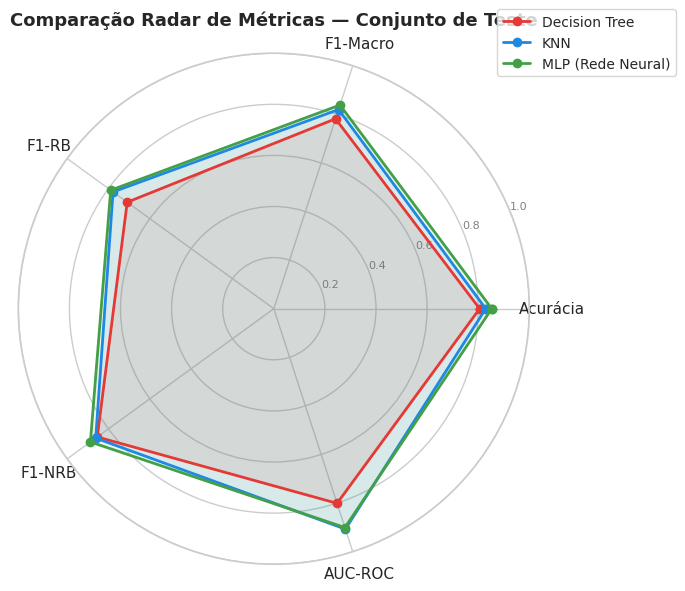
\includegraphics[width=0.6\textwidth]{fig_14_radar}
  \caption{Gráfico radar comparativo das métricas por modelo.}
  \label{fig:radar}
\end{figure}

\subsection{Modelagem Não Supervisionada}

O K-Means com $k=2$ obteve Inércia de 13.114,2 e Silhouette Score de
0,1635. O Cluster 1 concentrou 354 amostras NRB e 83 RB (81,0\% de
pureza NRB), enquanto o Cluster 0 ficou com 169 NRB e 193 RB (53,3\% RB).
O baixo Silhouette confirma sobreposição entre as classes no espaço
molecular --- coerente com o teto de 85,3\% atingido pelos modelos
supervisionados. A análise complementar com $k=5$ (Silhouette = 0,1724)
apresentou melhora marginal sem ganho interpretativo proporcional.
A variância explicada pelos dois componentes PCA usados na visualização
(Figura~\ref{fig:pca}) foi de 46,6\%, indicando que parte relevante
da estrutura dos dados ainda reside nas dimensões omitidas.

% ============================================================
\section{Análise Crítica Comparativa}
% ============================================================

\subsection{Por que certos modelos se saíram melhor ou pior}

O ordenamento MLP $>$ KNN $>$ Árvore de Decisão em F1-Macro
($0{,}838 > 0{,}820 > 0{,}782$) é consistente com as características
estruturais de cada algoritmo frente ao problema.

A \textbf{Árvore de Decisão} constrói fronteiras de decisão retangulares e
rígidas, inadequadas para descritores moleculares com relações contínuas e
sobrepostas entre classes. O F1-RB de 0,709 --- o mais baixo entre os três ---
evidencia maior dificuldade de capturar a classe minoritária, cujas regiões
no espaço de features são fragmentadas e não separáveis por divisões
ortogonais simples.

O \textbf{KNN} se beneficiou diretamente da normalização Z-Score: sem ela,
features com variância absoluta elevada (como \texttt{Me}, variância = 236.517)
dominariam o cálculo de distâncias. A distância Euclidiana com $k=5$ vizinhos
ponderados por distância revelou-se eficaz para capturar a estrutura local dos
dados normalizados. O alto recall de RB ($0{,}89$) indica boa sensibilidade à
classe minoritária, embora ao custo de maior taxa de falsos positivos (precisão-RB
= 0,69). A AUC-ROC de 0,907 --- a mais alta --- demonstra excelente capacidade de
ranqueamento.

A \textbf{MLP} atingiu o melhor F1-Macro ao modelar relações não lineares
complexas entre descritores. A arquitetura selecionada pelo 5-Fold CV foi
deliberadamente simples: 50 neurônios em camada única com regularização
$\alpha = 0{,}1$. Arquiteturas maiores estavam sobreajustando à variância do
treino --- o 5-Fold CV identificou esse overfitting e selecionou um modelo mais
parcimonioso. O perfil mais equilibrado entre NRB e RB (F1 de 0,889 e 0,789)
sugere que a rede aprendeu representações menos enviesadas para a classe
majoritária.

\subsection{Como o pré-processamento influenciou os resultados}

A normalização Z-Score foi crítica para KNN e MLP. A seleção de features por
importância RF capturou poder discriminativo distinto da simples variância:
9 das 20 features selecionadas têm variância abaixo do Top 20 por variância,
e os conjuntos se sobrepõem em apenas 50\%. A feature \texttt{Mi}, com a menor
variância do dataset ($0{,}0009$), foi selecionada por ser discriminativa,
ilustrando que variância e relevância preditiva são conceitos distintos.

O mapa de correlação das features selecionadas revelou alta colinearidade na
família SpMax/SM6 ($r > 0{,}91$). Essa redundância é tolerada por árvores de
decisão (que dividem sobre uma feature por vez), mas pode inflar artificialmente
a importância do grupo no cálculo de distâncias (KNN) e nos gradientes (MLP).

O SMOTE aplicado por fold no pipeline foi metodologicamente mais rigoroso do
que uma aplicação global. Na abordagem global, amostras sintéticas poderiam
ser geradas a partir de toda a base de treino e avaliadas como validação,
inflando as métricas de seleção de hiperparâmetros. Com o pipeline, cada fold
cria seus próprios sintéticos apenas com os dados disponíveis naquela iteração.

\subsection{Limitações do dataset}

O desbalanceamento de classes (66,4\%/33,6\%) é a principal limitação. Apesar
do SMOTE, todos os modelos apresentaram F1-RB consistentemente inferior ao
F1-NRB (gap de 10--15 pontos percentuais). O conjunto de teste preserva a
distribuição original e contém apenas 71 amostras RB --- cada erro pesa mais
nessa classe. A interpolação do SMOTE também pode não capturar toda a
diversidade estrutural das moléculas biodegradáveis reais.

A alta colinearidade na família SpMax/SM6 implica que o budget de 20 features
contém redundâncias que poderiam ser substituídas por descritores mais
independentes, potencialmente ampliando a diversidade de informação disponível
para os modelos.

\subsection{Em que medida os clusters fazem sentido}

O K-Means com $k=2$ recuperou parcialmente a estrutura binária sem supervisão:
o Cluster 1 apresentou 81,0\% de pureza NRB, resultado expressivo dado que o
algoritmo não teve acesso aos rótulos. O Silhouette Score baixo ($0{,}164$)
é consistente com o teto de performance supervisionada a 85,3\%: a dificuldade
de separação é intrínseca ao problema, não um artefato do K-Means.

\subsection{Se a estrutura não supervisionada ajuda a entender o problema}

Sim. A análise dos centroides revelou que os descritores que mais diferenciam
os clusters são exatamente os de maior importância no Random Forest --- índices
espectrais topológicos como SpMax e SM6. Isso indica coerência entre o que o
aprendizado não supervisionado descobre e o que os modelos supervisionados
utilizam para classificar. A existência de um cluster NRB com 81\% de pureza
apoia a hipótese de que moléculas estruturalmente mais complexas são menos
propensas à biodegradação, interpretação compatível com o conhecimento
químico sobre o tema.

% ============================================================
\section{Conclusão}
% ============================================================

Este trabalho abordou a predição de biodegradabilidade molecular por meio de
técnicas clássicas de aprendizado de máquina supervisionado e não supervisionado,
aplicadas ao dataset QSAR Biodegradation.

Na trilha supervisionada, a Rede Neural MLP demonstrou o melhor desempenho
geral, com acurácia de 85,3\%, F1-Macro de 0,838 e AUC-ROC de 0,901. O KNN
apresentou a maior AUC-ROC (0,907) e o melhor recall para a classe RB. A
Árvore de Decisão, apesar da maior interpretabilidade, ficou aquém dos demais
pela limitação estrutural de suas fronteiras de decisão frente à sobreposição
das classes.

Na trilha não supervisionada, o K-Means com $k=2$ recuperou parcialmente a
estrutura binária do problema sem acesso aos rótulos, com o Cluster 1
apresentando 81,0\% de pureza para NRB. O Silhouette Score baixo (0,164)
confirmou a sobreposição natural entre as classes, corroborando o teto de
performance observado nos modelos supervisionados.

As principais dificuldades foram o desbalanceamento de classes --- que persiste
mesmo após o SMOTE e impacta a detecção da classe RB --- e a multicolinearidade
entre descritores da família SpMax/SM6, que exige atenção na interpretação
das importâncias. O protocolo com 5-Fold CV e SMOTE por fold mostrou-se mais
rigoroso do que validações com split fixo.

Como aprendizados centrais, o trabalho reforçou: a importância da separação
estrita entre conjuntos desde o início do pipeline; a distinção entre variância
e relevância preditiva na seleção de features; e o valor da análise conjunta
de métricas --- acurácia isolada não captura o comportamento por classe em
problemas desbalanceados.

% ============================================================
\bibliographystyle{plainnat}
\bibliography{referencias}
% ============================================================

\end{document}
